In the burgeoning field of multimodal research, the integration of image understanding capabilities into large language models has become increasingly viable. 
Drawing inspiration from the open-sourced LLaVA~\citep{liu2023visual,liu2023improved}, we present Yi Vision Language (Yi-VL) models, \textit{i.e.}, Yi-VL-6B and Yi-VL-34B, based on Yi-6B-Chat and Yi-34B-Chat language models. 
The architecture of Yi-VL models, as illustrated in Figure \ref{fig:yi-vl}, comprises three primary modules. The Vision Transformer (ViT), used for image encoding, is initialized with CLIP ViT-H/14 model~\citep{ilharco_gabriel_2021_5143773}. A Projection Module, designed to align image features with text feature spcae, consists of a two-layer Multilayer Perceptron (MLP) with layer normalizations. Finally, the large language model, initialized with the Yi-Chat models, demonstrating exceptional proficiency in understanding and generating both English and Chinese. To enhance the performance of Yi-VL models in bilingual multimodal understanding and generation, we leverage a rich dataset of bilingual image-text pairs.

\begin{figure}[t]
    \centering
    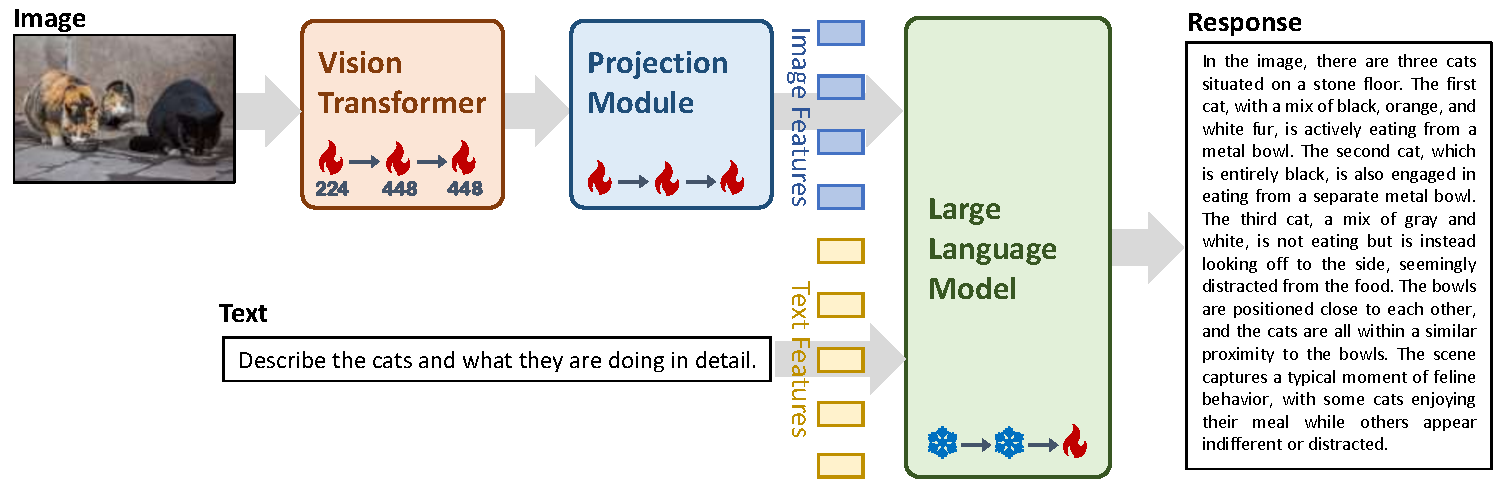
\includegraphics[width=0.98\textwidth]{images/yi-vl-cmmmu-1.pdf}
    \caption{Architecture of Yi-VL models. Symbols are used to denote the training status of various modules at three training stages: a fire icon (
\includegraphics[width=1em]{images/fire.png}) indicates the parameters of the module are trainable, while a snowflake icon (
\includegraphics[width=0.9em]{images/snow.png}) signifies that parameters are frozen. The image resolution used in ViT at each stage, either $224^2$ or $448^2$, is also marked.}
    \label{fig:yi-vl}
\end{figure}

Yi-VL models undergo a three-stage training process: 
\begin{description}[leftmargin=0.2in]
    \item[Stage 1:] we train the parameters of the ViT and the projection module using an image resolution of $224^2$. The training leverages a substantial dataset comprising $100$ million image-text pairs from LAION-400M~\citep{schuhmann2021laion}. The primary objective is to enhance the ViT's knowledge acquisition within our specified architecture and to achieve better alignment between the ViT and the LLM. 
    \item[Stage 2:] we scale up the image resolution of ViT to $448^2$, aiming to further boost the model's capability for discerning intricate visual details. The dataset used in this stage includes $20$ million image-text pairs derived from LAION-400M. Additionally, we incorporate around $4.8$ million image-text pairsn from diverse sources, \textit{e.g.}, CLLaVA~\citep{linksoulai2023chinesellava}, LLaVAR~\citep{zhang2023llavar}, Flickr~\citep{young2014image}, VQAv2~\citep{goyal2017making}, RefCOCO~\citep{kazemzadeh2014referitgame}, Visual7w~\citep{zhu2016visual7w} and so on.
    \item[Stage 3:] the parameters of the entire model are trained. The primary goal is to enhance the model's proficiency in multimodal chat interactions, thereby endowing it with the ability to seamlessly integrate and interpret visual and linguistic inputs. To this end, the training dataset encompasses a diverse range of sources, totalling approximately $1$ million image-text pairs, including GQA~\citep{hudson2019gqa}, VizWiz VQA~\citep{gurari2018vizwiz}, TextCaps~\citep{sidorov2020textcaps}, OCR-VQA~\citep{mishra2019ocr}, Visual Genome~\citep{krishna2017visual}, ShareGPT4V~\citep{chen2023sharegpt4v} and so on. To ensure data balancing, we impose a cap on the maximum data contribution from any single source, restricting it to no more than $50,000$ pairs. 
\end{description}

% \begin{itemize}
% \item In Stage 1, we train the parameters of the ViT and the projection module using an image resolution of $224^2$. The training leverages a substantial dataset comprising $100$ million image-text pairs from LAION-400M~\citep{schuhmann2021laion}. The primary objective is to enhance the ViT's knowledge acquisition within our specified architecture and to achieve better alignment between the ViT and the LLM. 

% \item In Stage 2, we scale up the image resolution of ViT to $448^2$, aiming to further boost the model's capability for discerning intricate visual details. The dataset used in this stage includes $20$ million image-text pairs derived from LAION-400M. Additionally, we incorporate around $4.8$ million image-text pairsn from diverse sources, \textit{e.g.},CLLaVA~\citep{linksoulai2023chinesellava}, LLaVAR~\citep{zhang2023llavar}, Flickr~\citep{young2014image}, VQAv2~\citep{goyal2017making}, RefCOCO~\citep{kazemzadeh2014referitgame}, Visual7w~\citep{zhu2016visual7w} and so on.

% \item In Stage 3, the parameters of the entire model are trained. The primary goal is to enhance the model's proficiency in multimodal chat interactions, thereby endowing it with the ability to seamlessly integrate and interpret visual and linguistic inputs. To this end, the training dataset encompasses a diverse range of sources, totalling approximately $1$ million image-text pairs, including GQA~\citep{hudson2019gqa}, VizWiz VQA~\citep{gurari2018vizwiz}, TextCaps~\citep{sidorov2020textcaps}, OCR-VQA~\citep{mishra2019ocr}, Visual Genome~\citep{krishna2017visual}, ShareGPT4V~\citep{chen2023sharegpt4v} and so on. to ensure data balancing, we impose a cap on the maximum data contribution from any single source, restricting it to no more than $50,000$ pairs. 
% \end{itemize}

In Stage 1 and 2, we set the global batch size, the learning rate, the gradient clip and the number of epoch to $4096$, $1$e$-4$, $0.5$ and $1$, respectively. In Stage 3, these parameters are adjusted to $256$, $2$e$-5$, $1.0$ and $2$. The training consumes $128$ NVIDIA A100 GPUs. The total training time amounted to approximately $3$ days for Yi-VL-6B and $10$ days for Yi-VL-34B. %We have made the Yi-VL models publicly available at \url{https://huggingface.co/01-ai/Yi-VL-6B} and \url{https://huggingface.co/01-ai/Yi-VL-34B}.

\begin{table}[t!]
\centering
\begin{tabular}{@{}lccccccc@{}}
\toprule
\textbf{Model}          & \textbf{Overall} & \textbf{Art} & \textbf{Business} & \textbf{Science} & \textbf{Health} & \textbf{Society} & \textbf{Engineering} \\ \midrule
GPT-4V & 55.7             & 65.3                   & 64.3              & 48.4             & 63.5                        & 76.3                         & 41.7                   \\
Yi-VL-34B               & 41.6             & 56.1                   & 33.3              & 32.9             & 45.9                        & 66.5                         & 36.0                   \\
Qwen-VL-PLUS            & 40.8             & 59.9                   & 34.5              & 32.8             & 43.7                        & 65.5                         & 32.9                   \\
Marco-VL                & 40.4             & 56.5                   & 31.0              & 31.0             & 46.9                        & 66.5                         & 33.8                   \\
Yi-VL-6B                & 37.8             & 53.4                   & 30.3              & 30.0             & 39.3                        & 58.5                         & 34.1                   \\
InfMIM-Zephyr-7B        & 35.5             & 50.0                   & 29.6              & 28.2             & 37.5                        & 54.6                         & 31.1                   \\
SVIT                    & 34.1             & 48.9                   & 28.0              & 26.8             & 35.5                        & 50.9                         & 30.7                   \\
Emu2-Chat               & 34.1             & 50.6                   & 27.7              & 28.0             & 32.4                        & 50.3                         & 31.3                   \\
BLIP-2 FLAN-T5-XXL       & 34.0             & 49.2                   & 28.6              & 27.3             & 33.7                        & 51.5                         & 30.4                   \\
InstructBLIP-T5-XXL      & 33.8             & 48.5                   & 30.6              & 27.6             & 33.6                        & 49.8                         & 29.4                   \\
LLaVA-1.5-13B            & 33.6             & 49.8                   & 28.2              & 25.9             & 34.9                        & 54.7                         & 28.3                   \\
Qwen-VL-7B-Chat          & 32.9             & 47.7                   & 29.8              & 25.6             & 33.6                        & 45.3                         & 30.2                   \\
SPHINX*                  & 32.9             & 50.9                   & 27.2              & 25.3             & 34.1                        & 51.2                         & 27.8                   \\
mPLUG-OWL2              & 32.1             & 48.5                   & 25.6              & 24.9             & 32.8                        & 46.7                         & 29.6                   \\
BLIP-2 FLAN-T5-XL        & 31.0             & 43.0                   & 25.6              & 25.1             & 31.8                        & 48.0                         & 27.8                   \\
InstructBLIP-T5-XL       & 30.6             & 43.3                   & 25.2              & 25.2             & 29.3                        & 45.8                         & 28.6                   \\
CogVLM                   & 30.1             & 38.0                   & 25.6              & 25.1             & 31.2                        & 41.5                         & 28.9                   \\ \bottomrule
\end{tabular}
\caption{\label{tab:yi_vl_mmmu}MMMU test set
 performance by the time of Yi-VL's release.}
\end{table}


Table~\ref{tab:yi_vl_mmmu} shows the MMMU test set leaderboard by Yi-VL's release. We note that this area is currently actively under research, aligning with the community's advances, we will continuously improve the update Yi-VL's performance. 